\documentclass[addpoints]{exam}
\usepackage{amsmath} % For math.
\usepackage{amsfonts} % For math fonts.
\usepackage{amssymb} % For other math symbols not covered by amsmath.
\usepackage[pdftex]{graphicx} % For pictures, use \includegraphics[scale=decimal]{pic.png}; must be a .png file type.
\usepackage{multicol}
\usepackage{textcomp}
%\usepackage{fullpage}
\usepackage{comment}
%\pdfpagewidth 8.5in
%\pdfpageheight 11in

%\setlength\topmargin{0in}
%%\setlength\headheight{0in}
%\setlength\headsep{0in}
%\setlength\textheight{10in}
%\setlength\textwidth{6.5in}
%\setlength\oddsidemargin{0in}
%\setlength\evensidemargin{0in}
%\setlength\parindent{0in}
%\setlength\parskip{.25in}

%\setlength\columnsep{0.3in}

\usepackage{tikz}
\usetikzlibrary{angles,quotes}
\usepackage{tkz-euclide}
\usetkzobj{all}

\newcommand{\ds}{\displaystyle}
\DeclareMathOperator{\dom}{{dom}}

\def\myrad{3cm}% radius of the circle
\def\myang{60}% angle for the arc

\begin{document}


\begin{flushleft}
Precalculus -  Exam \#2 \hfill  Name: \underline{\hspace{2.5 in}} \\  
  \hfill  Section \# (or meeting time):  \underline{\hspace{1in}}\\  %\hspace{0.0025in} \\
%\hspace*{0.25in} 
Make sure to show all work to receive full credit  \hfill  Score: \underline{\hspace{0.5in}} out of 48 \\
{\bf Important}: Leave all answers as an \underline{\bf exact} value unless otherwise stated.
\end{flushleft}


\begin{questions}


\question[3]
Solve $\log_4(x-2)=5$ for $x$.

\vfill

\noindent\makebox[\linewidth]{\rule{\paperwidth}{0.4pt}}
\question[5]
Solve $2\cdot 4^{3x-4} =10$.

\vfill


%\vspace*{-2em}
\question[3] On the day of a child's birth, a parent deposits \$10,000 in a trust fund that pays 10\% interest, compounded continuously. Determine the balance in this account on the child's $18^{th}$ birthday. (Round your answer to two decimal places.)


%\question[5] Solve $5(4^x)=35$ for $x$. 
\vfill
\pagebreak

\question[5]
Determine if $\left(\dfrac{\sqrt{13}}{7},\dfrac{6}{7}\right)$ is on the unit circle.

\vfill
%\question[5]  Solve $\ln(2x+1)=4$ for $x$. 

%\question[5] Write $3\ln(x) + \frac{1}{2}\ln(y) -4\ln(x^2+y)$ as a single logarithm.


\question[5]
Determine the principal $P$ that must be invested at rate $r = 8\%$, compounded monthly, so that \$500,000 will be available for retirement in $t = 40$ years. (Round your answer to the nearest cent.)

\vfill

%\question[5] Solve $e^{2x}-e^x-6=0$ for $x$.

\question
Perform the conversion below.\\
\begin{tabular}{l|l}

a. (2 points) Convert $135^{\circ}$ degrees to radians & b. (2 points) Convert $\dfrac{2\pi}{3}$ radians to degrees\\
&\\
&\\
&\\
&\\
&\\
&\\
&\\
&\\
&\\
&\\
&\\
&\\
&\\
&\\
&\\
\end{tabular}

\pagebreak

\question[2]
Find any angle (other than the angle itself) that is coterminal with $\dfrac{7\pi}{6}$.
\vfill
%\vspace*{-2em}

\noindent\makebox[\linewidth]{\rule{\paperwidth}{0.4pt}}
\question[3] A $7\frac{1}{4}$-inch circular power saw blade rotates at 5200 revolutions per minute.  Find the linear speed (in feet per minute) of the saw teeth as they contact the wood being cut.
%\question[3]
%Find the reference angle for $\theta=\dfrac{29\pi}{6}$.
\vfill
%\vspace*{-2em}


\noindent\makebox[\linewidth]{\rule{\paperwidth}{0.4pt}}
\question [3]
Evaluate $\cos \left(\dfrac{7\pi}{6}\right)$.

\vfill

\noindent\makebox[\linewidth]{\rule{\paperwidth}{0.4pt}}
\question[5] Write $3\ln(x) + \frac{1}{2}\ln(y) -4\ln(x^2+y)$ as a single logarithm.
\vfill
%\vspace*{-2em}

\vfill
\pagebreak

\begin{comment}
\question
Given the triangle below, evaluate
\begin{parts}
\part[2]  $\tan \theta$.
\part[2] $\sec \theta$.
\end{parts}
\begin{flushleft}

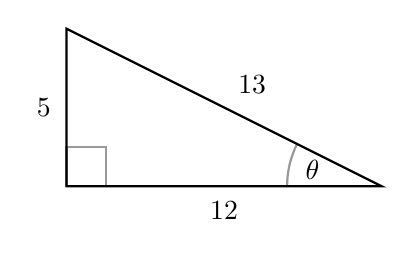
\begin{tikzpicture}[thick]
\coordinate (O) at (0,0);
\coordinate (A) at (4,0);
\coordinate (B) at (0,2);
\draw (O)--(A)--(B)--cycle;

\tkzLabelSegment[below=2pt](O,A){\text{12}}
\tkzLabelSegment[left=2pt](O,B){\text{5}}
\tkzLabelSegment[above right=2pt](A,B){\text{13}}

\tkzMarkRightAngle[size=0.5,opacity=.4](A,O,B)% square angle here
%\tkzLabelAngle[pos = 0.35](A,O,B){$\gamma$}

\tkzMarkAngle[size=1.2cm,%
opacity=.4](B,A,O)
\tkzLabelAngle[pos = 0.9](B,A,O){$\theta$}

\end{tikzpicture}
\end{flushleft}

\vspace*{-2em}
\noindent\makebox[\linewidth]{\rule{\paperwidth}{0.4pt}}
\end{comment}


\question[5]
Find the area of the sector defined by $\theta$ below.\\
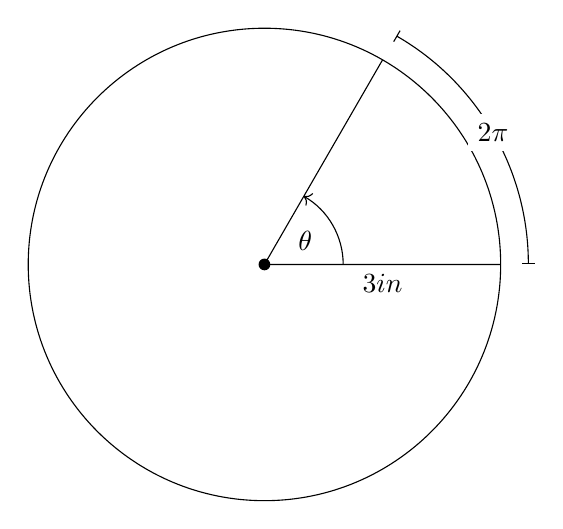
\begin{tikzpicture}
% the origin
\coordinate (O) at (0,0);
% the circle and the dot at the origin
\draw (O) node[circle,inner sep=1.5pt,fill] {} circle [radius=\myrad];
% the ``\theta'' arc
\draw 
  (\myrad,0) coordinate (xcoord) -- 
  node[midway,below] {$3in$} (O) -- 
  (\myang:\myrad) coordinate (slcoord)
  pic [draw,->,angle radius=1cm,"$\theta$"] {angle = xcoord--O--slcoord};
% the outer ``s'' arc
\draw[|-|]
  (\myrad+10pt,0)
  arc[start angle=0,end angle=\myang,radius=\myrad+10pt]
  node[midway,fill=white] {$2\pi$};
\end{tikzpicture}

%\vspace*{-2em}

$ \dfrac{1}{x} |_{x=1} $


\vspace{8em}

%\question[5] A building casts a shadow of $230$ feet long.  Find the height of the building if the angle of elevation of the Sun is $23.6^{\circ}$.  Approximate to the nearest foot.

%\vfill
\noindent\makebox[\linewidth]{\rule{\paperwidth}{0.4pt}}
\question[5]
Find all vertical, horizontal and/or oblique (slant) asymptotes that exist of the graph of the function $f(x)=\dfrac{x^2-7x-8}{4x^2+x-3}$.

\vfill

\end{questions}

\pagebreak

\begin{center}
\LARGE  Formulas
\end{center}

\noindent $A=P\left( 1+\dfrac{r}{m}\right) ^ {mt}$\\ \\
$A=Pe^{rt}$\\ \\
$A=\dfrac{1}{2}r^2\theta$\\ \\
$\omega=\dfrac{\theta}{t}$\\ \\
$v=\dfrac{\theta\cdot r}{t}$\\ \\
$n(t)=n_0e^{rt}$\\ \\
$m(t)=m_0e^{-rt}$  where $\frac{\ln(2)}{h}$\\ \\
$\log_b z=y$ iff $b^y=z$\\ \\


\noindent 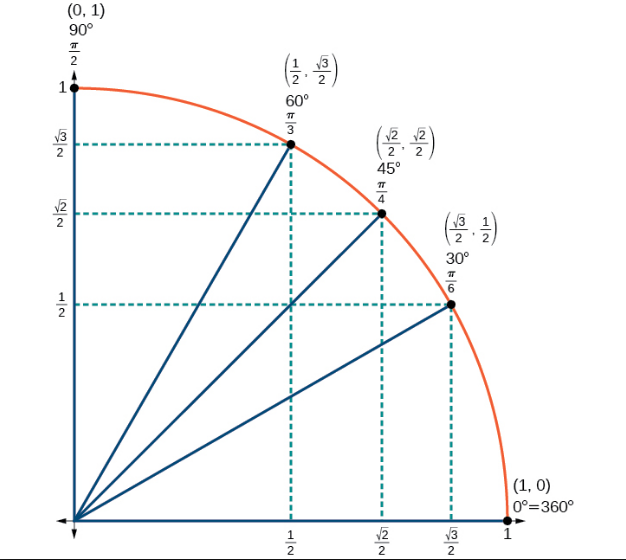
\includegraphics[width=5in]{pic1.png}



\end{document}





























